\documentclass{article}
\usepackage[utf8x]{inputenc}
\usepackage[colorlinks=true,linkcolor=black,citecolor=blue,pdfusetitle,pagebackref=false]{hyperref}
\usepackage[nonumberlist]{glossaries}
\usepackage{graphicx}
\usepackage{multicol}
\usepackage{caption}
\usepackage{subcaption}
\usepackage{authblk}
\usepackage{amsmath}
\usepackage{bm}
\usepackage[margin=1.5cm]{geometry}
\usepackage{cite}
\usepackage[usenames,dvipsnames,svgnames,table]{xcolor}
\usepackage{bigints}

\newenvironment{Figure}
  {\par\medskip\noindent\minipage{\linewidth}}
  {\endminipage\par\medskip}

\bibliographystyle{unsrt}
\renewcommand\refname{References}

\newacronym{cdi}
    {CDI}{coherent diffractive imaging}

\newacronym{odt}
    {ODT}{optical dipole trap}

\newacronym{bec}
    {BEC}{Bose-Einstein condensate}

\newacronym{fort}
    {FORT}{far-off-resonance trap}

\newacronym{ta}
    {TA}{tapered amplifier}

\newacronym{caes}
    {CAES}{cold-atom electron source}

\newacronym{xfel}
    {XFEL}{x-ray free electron laser}

\newacronym{mot}
    {MOT}{magneto-optical trap}

\newacronym{ecdl}
    {ECDL}{external cavity diode laser}

\newacronym{aom}
    {AOM}{acousto-optical modulator}

\newacronym{slm}
    {SLM}{spatial light modulator}

\newacronym{mopa}
    {MOPA}{master-oscillator power amplifier}

\newacronym{na}
    {NA}{numerical aperture}

\newacronym{ar}
    {AR}{anti-reflection}

\newacronym{ccd}
    {CCD}{charge-coupled device}

\newacronym{cro}
    {CRO}{cathode ray oscilloscope}

\newacronym{pbs}
    {PBS}{polarising beam splitter}

\newacronym{bs}
    {BS}{beam splitter}

\newacronym{npbs}
    {NPBS}{non-polarising beam splitter}

\newacronym{tec}
    {TEC}{thermo-electric cooler}

\newacronym{cw}
    {CW}{continuous wave}

\newacronym{mcp}
    {MCP}{microchannel plate}

\newacronym{fwhm}
    {FWHM}{full-width half maximum}

\newacronym{pdh}
    {PDH}{Pound-Drever-Hall}
    
\newacronym{ps}
    {PS}{polarisation spectroscopy}
    
\newacronym{obe}
    {OBE}{optical Bloch equation}
    
\newacronym{davll}
    {DAVLL}{dichroic atomic vapour laser lock}

\newacronym{mts}
    {MTS}{modulation transfer spectroscopy}

\newacronym{snr}
    {SNR}{signal-to-noise ratio}

\newacronym{lsd}
    {LSP}{linear spectral density}


\makeglossaries

\begin{document}
\title{kHz linewidth lasers using atomic coherence}
\author[1]{J. S. J. Torrance}
\author[1]{B. M. Sparkes}
\author[1]{R. E. Scholten}

\affil[1]{School of Physics, The University of Melbourne, Melbourne, Victoria 3010 Australia}

\maketitle

\begin{abstract}
By capitalising on the demonstrably high bandwidth of polarisation spectroscopy locking systems it it possible to achieve linewidths of less than 1\,kHz using standard diode lasers.
\end{abstract}

\begin{multicols}{2}

\section{Intro}
Laser frequency stabilisation to atomic references is essential to numerous applications including the cooling and trapping of atoms\cite{uetake_high_2008, ye_stable_2010, akamatsu_narrow_2012}, atomic clocks\cite{ludlow_sr_2008}, high resolution spectroscopy\cite{rafac_sub-dekahertz_2000} and metrology\cite{metcalf_laser_1999, ye_quantum_2008, demtroder_laser_2014}. Narrow linewidth lasers are also important to {\color{red}blah blah}.

Current techniques for minimising laser linewidths range from laser stabilisation with saturated absorption spectroscopy, which can achieve linewidths in the region of 150\,kHz\cite{cuneo_optically_1994}, to elaborate experiments involving extremely high finesse cavities that are able to achieve sub-Hertz linewidths with diode lasers using \gls{pdh} locking\cite{ludlow_compact_2007}.

\Gls{ps}\cite{wieman_doppler-free_1976, demtroder_laser_2014} has much in common with saturated absorption spectroscopy\cite{maguire_theoretical_2006, haroche_theory_1972, preston_doppler-free_1996} as both techniques provide frequency stabilisation to atomic references however \gls{ps} is shown here to be able to reduce diode laser linewidths to kHz levels.

It has been shown that \gls{ps} can be used to reduce the linewidth of a distributed feedback diode from 2\,MHz to 20\,kHz\cite{torii_laser-phase_2012}. Diode lasers locked with \gls{ps} have previously reported wavelengths of 65\,kHz\cite{yoshikawa_frequency_2003}. Our \gls{ps} locking system utilises high bandwidth feedback to the laser diode to achieve linewidths of order 1\,kHz.

\section{Pol Spec Theory}

\Gls{ps} uses counterpropagating pump and probe beams from the same laser in order to induce birefringence in an atomic sample. The circularly polarised pump beam induces circular birefringence in the sample while the linearly polarised probe beam is rotated by the birefringence\cite{wieman_doppler-free_1976, demtroder_laser_2014}. This results in an error signal ideal for laser locking.

The polarisation rotation of the probe can be monitored using a balanced polarimeter which consists of a quarter-wave plate, \gls{pbs} and two high-bandwidth detectors. A balanced polarimeter provides a background-free signal which is ideal for laser locking\cite{pearman_polarization_2002}. An schematic of polarisation spectroscopy with a balanced polarimeter is shown in figure \ref{polspec_schematic} and an example of a \gls{ps} error signal is given in figure \ref{polspec_spectrum}.

The refractive index of a pumped atomic sample is given by\cite{sheludko_shaped_2010}
\begin{align}
n=1+N\frac{\sigma_0\lambda}{4\pi}\frac{\Gamma}{\Omega_{ge}}\rho_{ge}
\end{align}
where $N$ is the atomic density of the sample, $\sigma_0$ is the atomic cross-section, $\lambda$ is the wavelength of the light, $\Omega_{ge}$ is the Rabi frequency for the transition in question and $\rho_{ge}$ is the off-diagonal element of the density matrix derived from the \glspl{obe}.

The polarisation rotation of the probe beam can be described by\cite{hecht_optics_1987}
\begin{align}
\Delta\theta=\frac{\pi L}{\lambda}(n_+-n_-)
\end{align}
where $L$ is the length of the atomic sample and $n_\pm$ are the refractive indices for the circularly polarised components of the linear probe beam.

If we integrate over the velocities of the atomic sample {\color{red}then we get something that looks like figure \ref{dispersion}}

\begin{Figure}
    \centering
    \captionsetup{type=figure}
    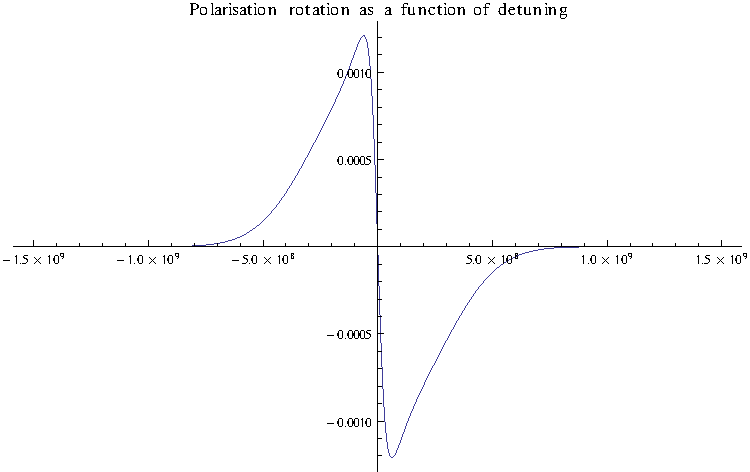
\includegraphics[width=0.75\linewidth]{Figs/dispersion.pdf}
    \captionof{figure}{The rotation of the probe beam as it passes through an atomic sample pumped by the pump beam as the detuning of the laser is scanned over the atomic resonance.}
    \label{dispersion}
\end{Figure}

The polarisation rotation of the probe beam produces the error signal that is sued to lock the laser. Unlike saturated absorption spectroscopy, where reaction time of the error signal is limited by the lifetime of the excited state atoms, the \gls{ps} error signal depends solely on the interaction of the light with the refractive index and thus the reaction time of the error signal is only limited by technical considerations and noise.

\begin{Figure}
    \centering
    \captionsetup{type=figure}
    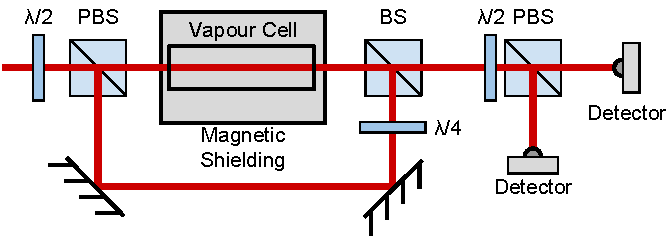
\includegraphics[width=\linewidth]{Figs/PolSpec.pdf}
    \captionof{figure}{Polarisation spectroscopy with a balanced polarimeter.}
    \label{polspec_schematic}
\end{Figure}

\begin{Figure}
    \centering
    \captionsetup{type=figure}
    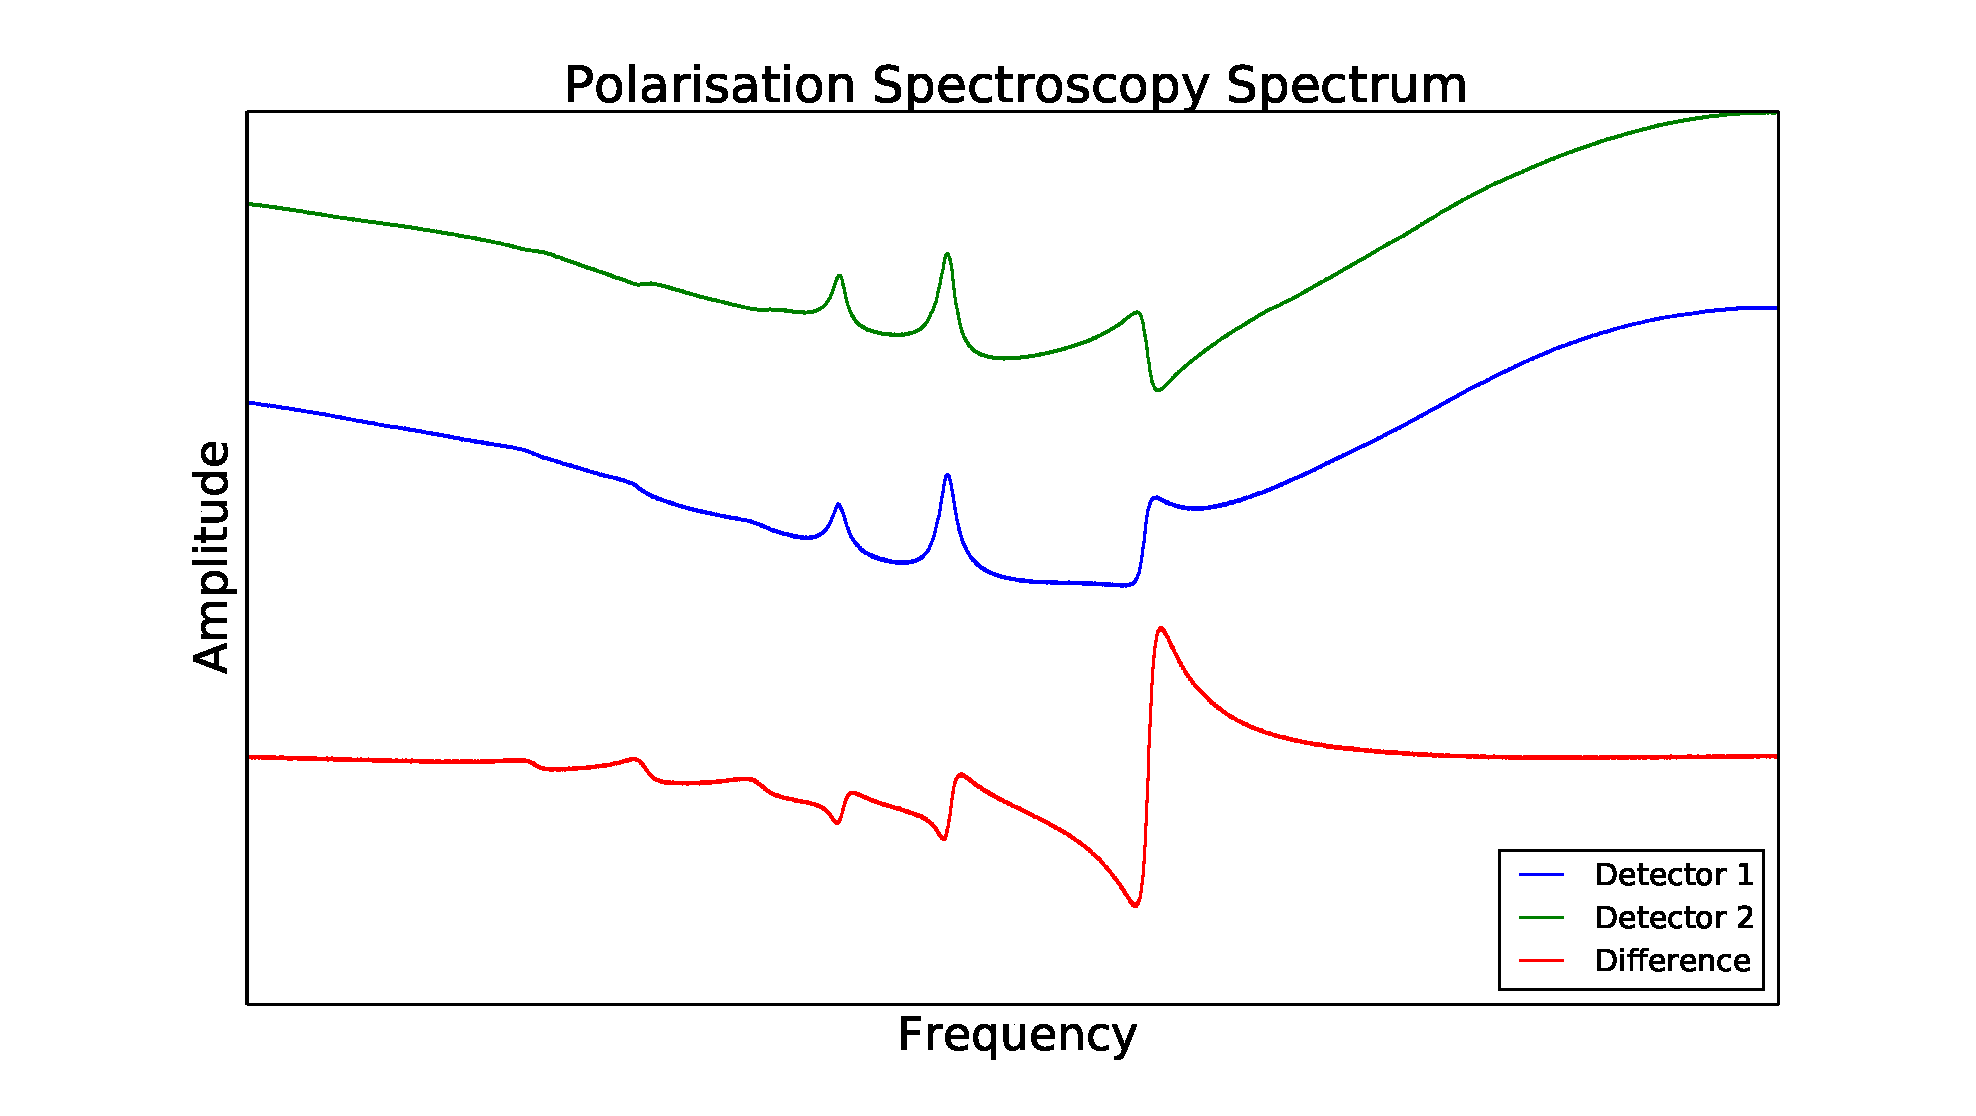
\includegraphics[width=\linewidth]{Figs/spectrum.pdf}
    \captionof{figure}{An example of the polarisation spectrum of the Rb85 cooling transition. This is a stand in image. One showing pol spec vs sat abs would probably be more useful. Label the various transitions too.}
    \label{polspec_spectrum}
\end{Figure}

\section{Setup}

The experimental setup is depicted in figure \ref{polspec_full_schematic}. Two separate \glspl{ecdl} were individually locked using \gls{ps} and high bandwidth feedback. A heterodyne measurement was then taken to determine the lasers' spectral linewidths.

\begin{Figure}
    \centering
    \captionsetup{type=figure}
    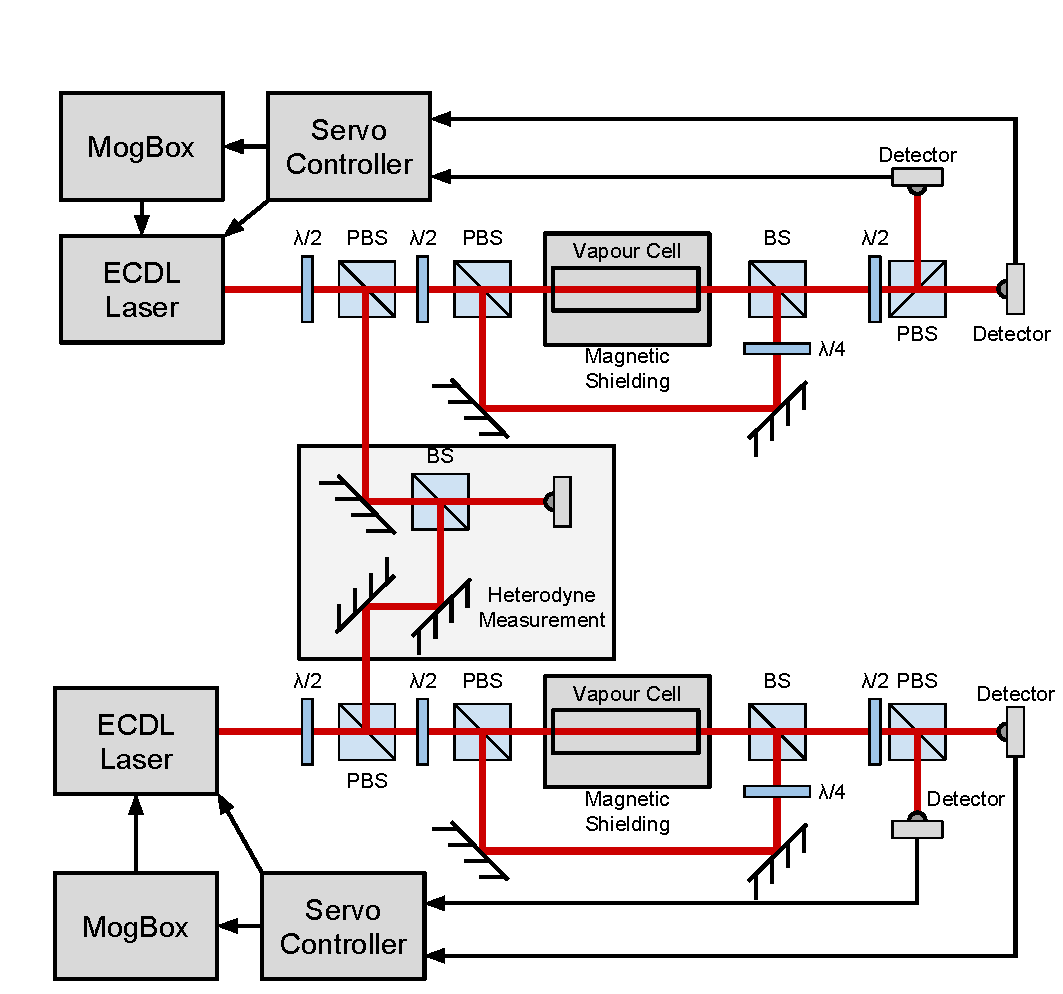
\includegraphics[width=\linewidth]{Figs/FullSimplifiedPolSpecSchematicAttempt.pdf}
    \captionof{figure}{A schematic diagram of the \gls{ps} setup. This is pretty ugly. Needs work.}
    \label{polspec_full_schematic}
\end{Figure}

High bandwidth feedback is achieved using high bandwidth detectors in the balanced polarimeter (ThorLabs PDA10A-EC with a bandwidth of 100\,MHz), a high bandwidth servo controller (NewFocus LB1005 with a bandwidth of 18\,MHz) and high bandwidth modulation inputs to the laser diodes (DC to 100\,MHz on the Toptica DL Pro and {\color{red} something else} on the MOGLabs ECDL via a customised headboard).

Isolating the laser diode from the electrical ground plane {\color{red} via some arcane arrangements of FETs as shown in a figure \ref{FET_circuit}} is essential in order to reduce the noise in the current modulation of the diode.

\begin{Figure}
    \centering
    \captionsetup{type=figure}
    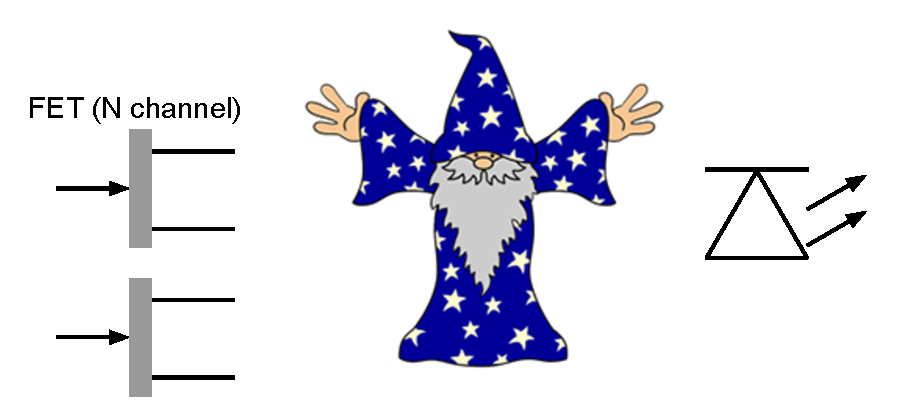
\includegraphics[width=\linewidth]{Figs/LaserDiodeAndFETs.pdf}
    \captionof{figure}{A simplified schematic diagram of the MOG laser FET setup. {\color{red}May not be 100\% accurate.}}
    \label{FET_circuit}
\end{Figure}

\begin{itemize}
\item let's not bother mentioning the fibres except perhaps in passing if long term drift is mentioned
\end{itemize}


\begin{itemize}
\item describe linewidth measurements
    \begin{itemize}
    \item beatnote - standard measurement, probably no need to go into detail
    \end{itemize}
\end{itemize}


\section{Results}
\subsection{Bandwidth}
The bandwidth of \gls{ps} can be determined by looking at the spectrum of the error signal on- and off-resonance. The frequency where the two spectra cross indicates the bandwidth of \gls{ps}. As shown in figure \label{bandwidth_measurement} the bandwidth for the Toptica laser and it's \gls{ps} setup is 58\,MHz. {\color{red} 58\,MHz is the first zero crossing of the moving average. The first crossing of the raw data is around 30\,MHz which is still respectable.}

{\color{red} This bandwidth means that this setup is capable of achieving linewidths of what? How do I work this out?}

\begin{Figure}
    \centering
    \captionsetup{type=figure}
    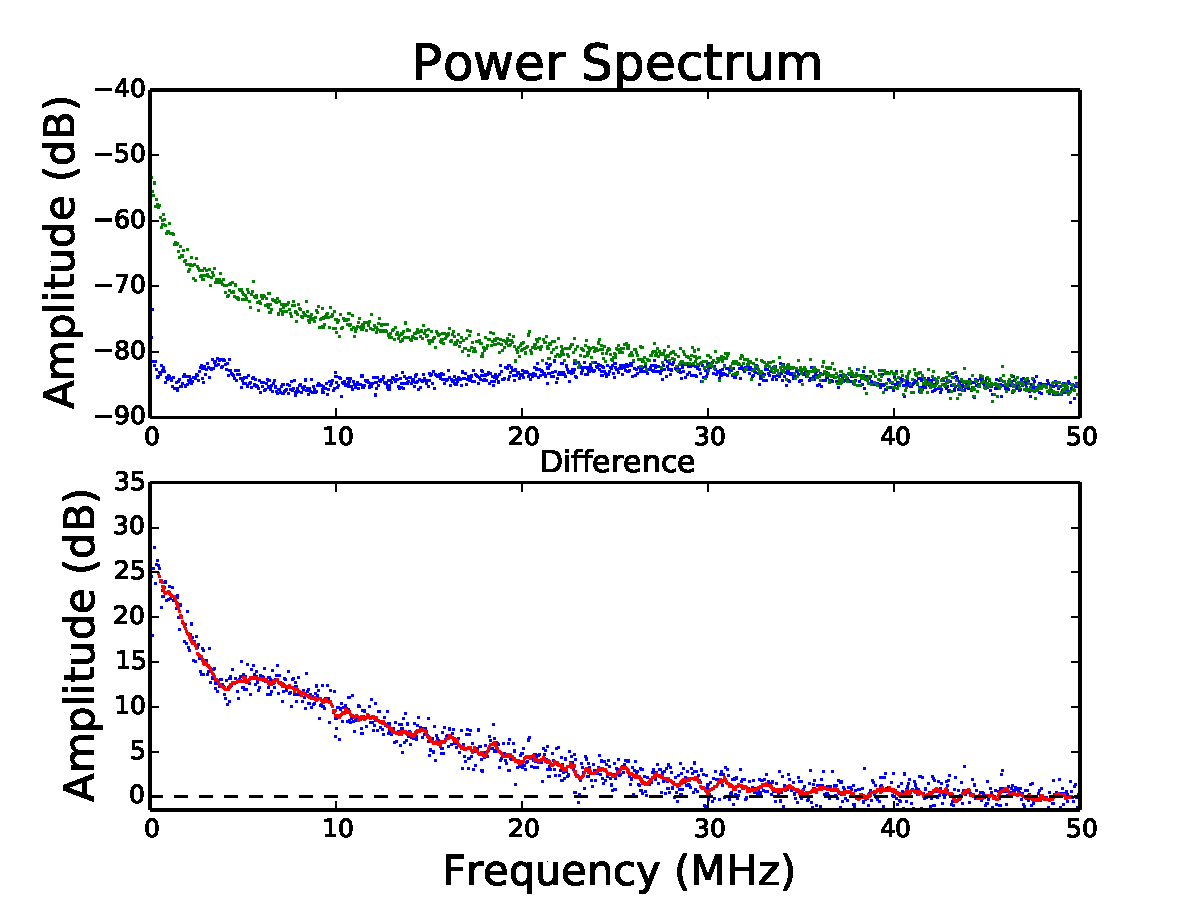
\includegraphics[width=\linewidth]{Figs/bandwidth.pdf}
    \captionof{figure}{Bandwidth measurement of the Toptica \gls{ps} setup. This figure needs prettifying}
    \label{bandwidth_measurement}
\end{Figure}

\subsection{Heterodyne Measurements}

\begin{Figure}
    \centering
    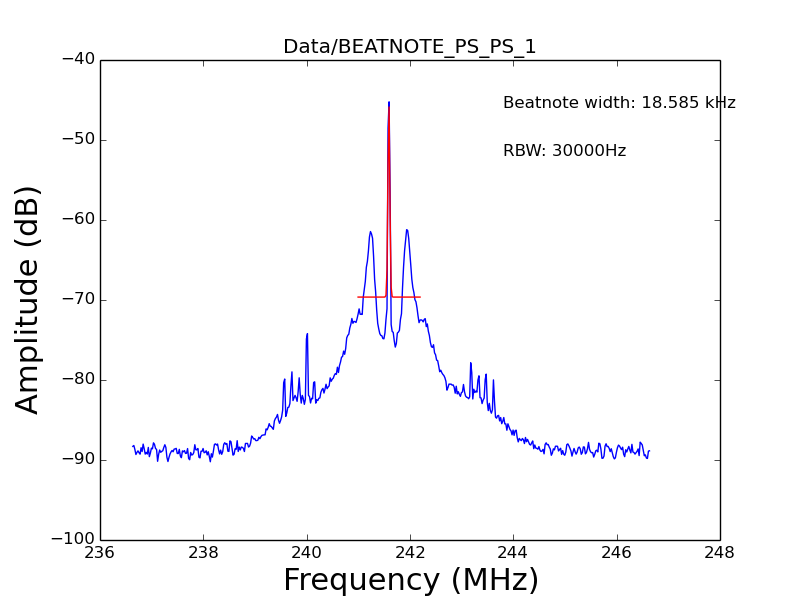
\includegraphics[width=0.49\linewidth]{Figs/beatnote_wide.png}
    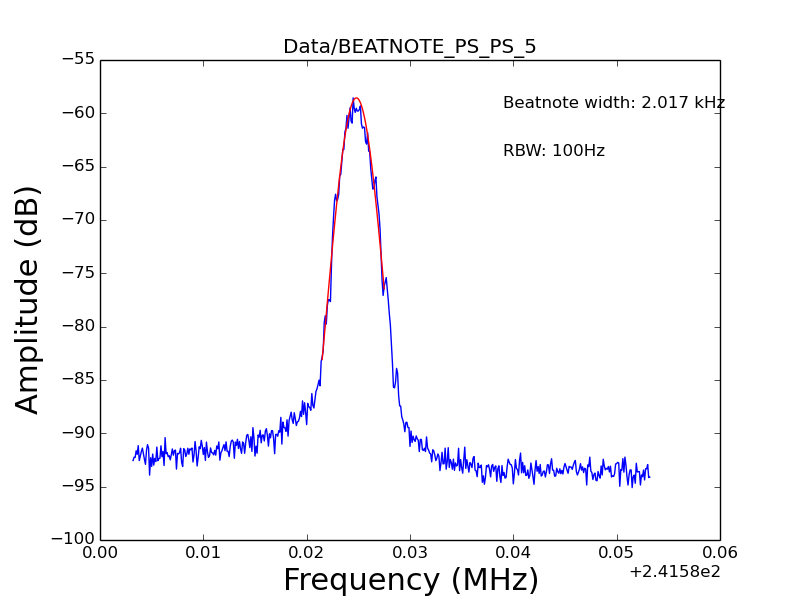
\includegraphics[width=0.49\linewidth]{Figs/beatnote_zoom.png}
    \captionsetup{type=figure}
    \captionof{figure}{Typical heterodyne beatnotes for the two lasers locked with \gls{ps}. Both measurements are 50 shot averages taken one after the other.}
    \label{beatnote}
\end{Figure}

\begin{itemize}
\item cavity linewidth measurements
\item beatnote to individual laser linewidth
\item remaining jitter
\item mechanical stability of the MogLaser is the current limiting factor
\end{itemize}

\section{Things to consider}
\begin{itemize}
\item Replicate numerical solution in \cite{harris_polarization_2006}?
\item Transient temperature/frequency drift - possible solution with intensity stabilisation.
\item What about phase lead? I didn't end up using any I think.
\item Things that perhaps should be mentioned:
    \begin{itemize}
    \item cost advantage
    \item broad locking range
    \item good signal to noise
    \end{itemize}
\end{itemize}

\section{Acknowedgements}
\begin{itemize}
\item Alex for electronics help (or should he be an author?)
\item Rory for sanity checking of code
\end{itemize}

\bibliographystyle{plain}
\bibliography{Library}

\end{multicols}
\end{document}
